\chapter*{Introduction}
\addcontentsline{toc}{chapter}{Introduction}

Let us introduce two combinatorial problems:

\begin{prob-intro}
\label{prob:table}
Consider a table of addition modulo $n$; it is a latin square $n \times n$. What is the smallest number of cells that we have to change in order to get another latin square?
\end{prob-intro}

\begin{figure}[htb]
	\centering
	\begin{minipage}{.40\linewidth}
		\begin{center}
		\begin{tabular}{| c c c c c c c |}
			\hline
			\M0 & 1 & 2 & \M3 & 4 & 5 & 6 \\
			1 & 2 & 3 & 4 & 5 & 6 & 0 \\
			2 & 3 & 4 & 5 & 6 & 0 & 1 \\
			\M3 & 4 & \M5 & \M6 & 0 & 1 & 2 \\
			4 & 5 & \M6 & \M0 & 1 & 2 & 3 \\
			\M5 & 6 & \M0 & 1 & 2 & 3 & 4 \\
			6 & 0 & 1 & 2 & 3 & 4 & 5 \\
			\hline
		\end{tabular}
		\end{center}	\end{minipage}
	$\longrightarrow$
	\begin{minipage}{.40\linewidth}
		\begin{center}
		\begin{tabular}{| c c c c c c c |}
			\hline
			\M3 & 1 & 2 & \M0 & 4 & 5 & 6 \\
			1 & 2 & 3 & 4 & 5 & 6 & 0 \\
			2 & 3 & 4 & 5 & 6 & 0 & 1 \\
			\M5 & 4 & \M6 & \M3 & 0 & 1 & 2 \\
			4 & 5 & \M0 & \M6 & 1 & 2 & 3 \\
			\M0 & 6 & \M5 & 1 & 2 & 3 & 4 \\
			6 & 0 & 1 & 2 & 3 & 4 & 5 \\
			\hline
		\end{tabular}
		\end{center}
	\end{minipage}
	\caption{The smallest number for $n=7$ is nine.}
\end{figure}

\begin{prob-intro}
\label{prob:triangle}
Let $\Delta_n$ be an equilateral triangle of side $n$. What is the smallest number of integer-sided equilateral triangles, into which $\Delta_n$ can be dissected, such that no six of them share a common point?
\end{prob-intro}

\begin{figure}[htb]
\centering
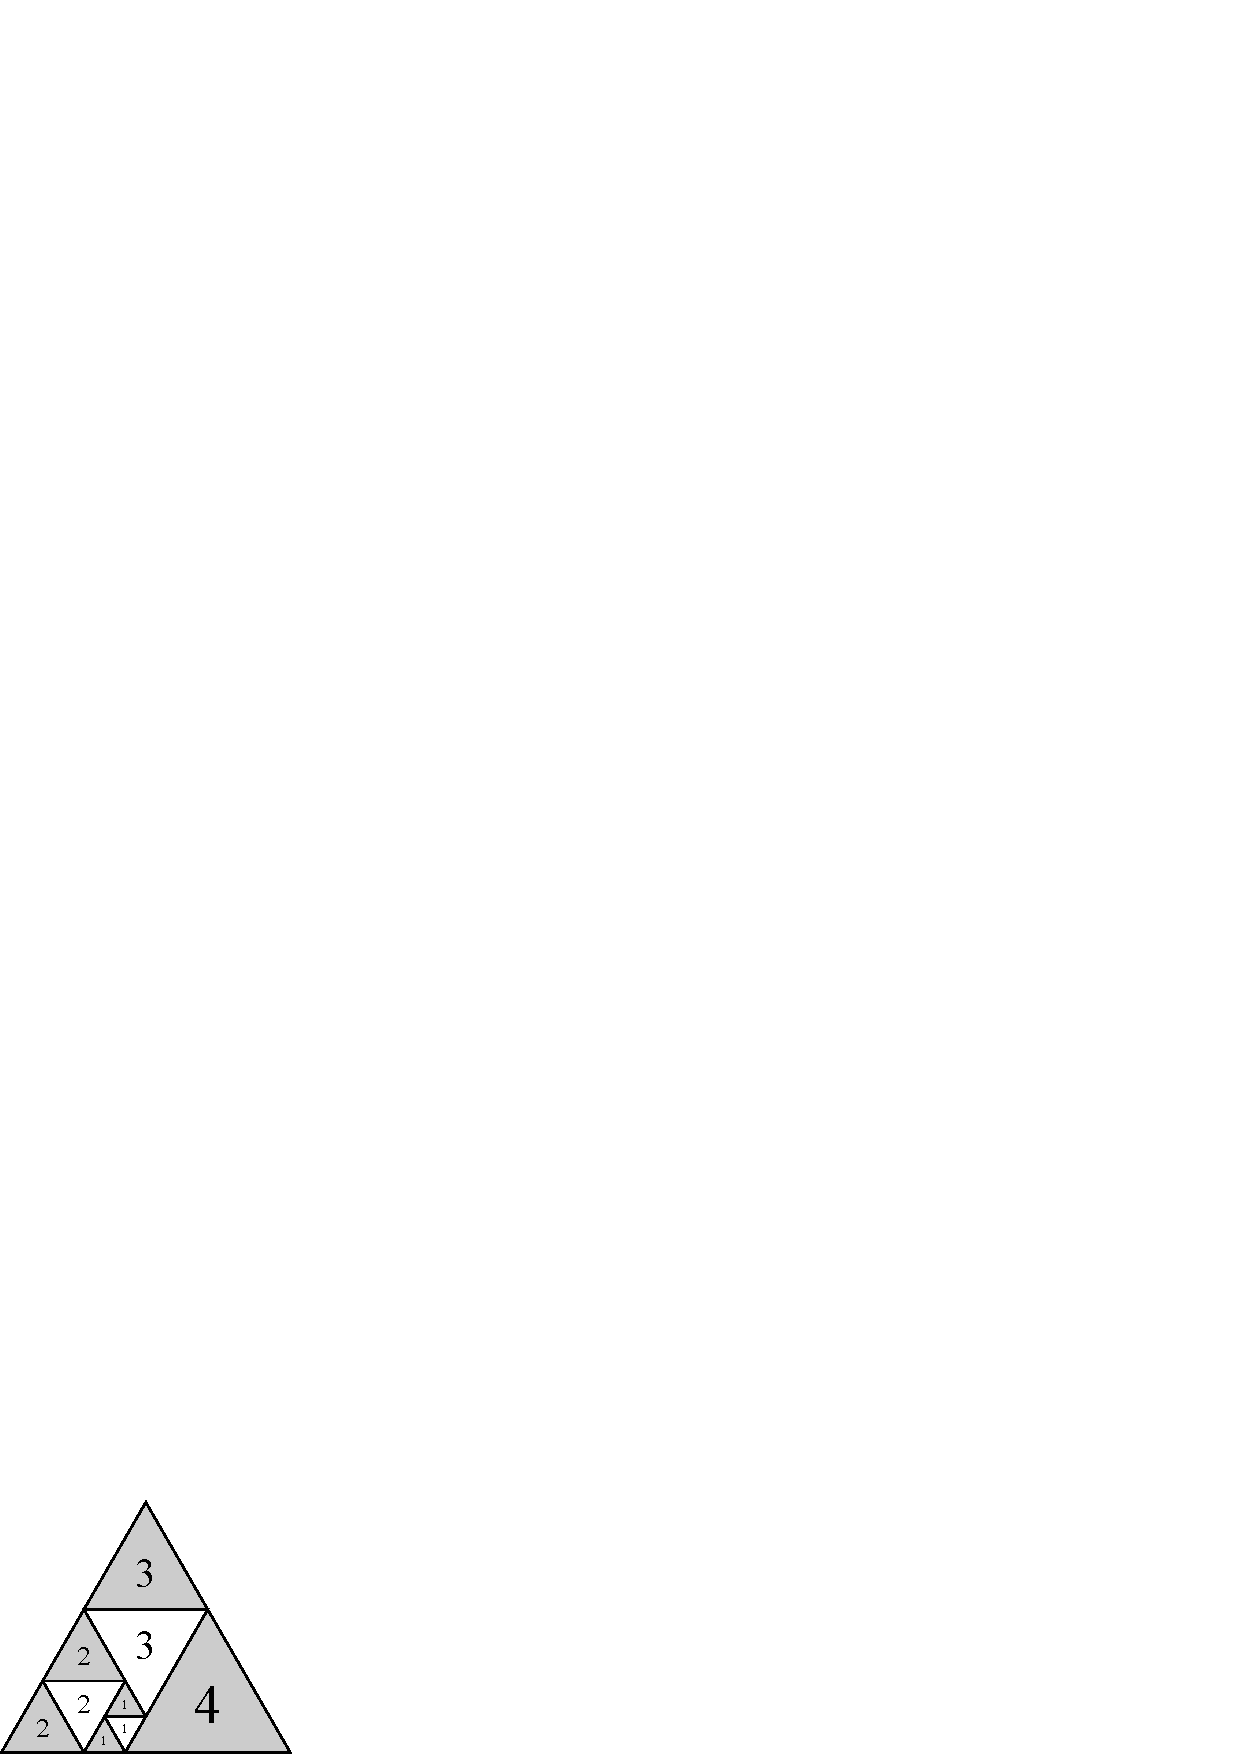
\includegraphics[width=0.35\textwidth]{img/dissection7.pdf}
\caption{Dissection of a triangle of size 7 into nine triangles.}
\label{fig:dissection7}
\end{figure}

Though it is not obvious at first glance, these two problems are fundamentally related. Both triangle dissections and pairs of latin squares describe a combinatorial structure called \emph{latin bitrade}. This structure will be of central interest throughout this work.

Let us denote by $\gdist(n)$ and $t(n)$ the minimal numbers described in Problems \ref{prob:table} and \ref{prob:triangle} respectively. Our main result is a solution to the twenty-year-old conjecture of Drápal, Cavenagh and Wanless:

\begin{conj-intro}
\label{conj:main}
There exist positive constants $c_1$ and $c_2$ such that
\begin{cosyeqnarray}
	c_1 \log(p) \leq \gdist(p) \leq c_2 \log(p) \label{eq:conj1}
\end{cosyeqnarray}
for sufficiently large primes $p$.
\end{conj-intro}

In other words, the conjecture states that $\gdist(n)$ is asymptotically logarithmic, the condition for $n$ to be a prime is only a technical requirement. We also prove the same statement for $t(n)$ in place of $\gdist(n)$.

The lower bound in (\ref{eq:conj1}) was already established before. In 1989 Drápal and Kepka~\cite{DrapalKepka89} proved the inequality for $c_1 = e$, and later Cavenagh~\cite{Cavenagh03} found an alternative proof of the same estimate. Yet another proof was given in a paper~\cite{CavenaghWanless09} by Cavenagh and Wanless, but with a slightly smaller constant.

All of these proofs are dealing with another structure which defines a latin bitrade -- certain kind of 0-1 matrices. The lower bound is then determined by establishing upper bound for determinant of such a matrix. In Chapter \ref{chap:lower-bound} we present modified proof which leads to $c_1 = 3 \log_3(e)$, the best estimate known so far.

\bigskip

The previously known best upper bound $\gdist(p) = O(\log^2(p))$ is due to Drápal~\cite{Drapal91}. He discovered the connection between latin bitrades and dissections of equilateral triangles, and proved that $\gdist(n) \leq t(n)$. However, he was only able to construct triangle dissections with $O(\log^2(n))$ triangles.

In Chapter \ref{chap:dissections} we prove Conjecture~\ref{conj:main} by constructing dissections into logarithmically many triangles. The method used is inspired by Trustrum's method \cite{Trustrum65} to  dissect a square of side $n$ into logarithmically many integer-sided squares. To be more precise, we show how to dissect an $n \times (n+3)$ rectangle into $5 \log_4(n) + \frac{3}{2}$ squares and how to adapt the construction to get a dissection of an equilateral triangle of side $n$ into $5 \log_2(n)$ triangles. We also discuss possible generalizations of our dissection method in Section \ref{sec:other-log-dissections}.

\bigskip

Now, that the asymptotic behavior of $\gdist(n)$ and $t(n)$ is known, it is natural to ask about the constants in the estimates. Putting our results together, we get
\begin{eqnarray}
	2.73 \approx 3 \log_3(e) \leq \frac{\gdist(p)}{\log(p)} \leq \frac{t(p)}{\log(p)} < 5 \log_2(e) \approx 7.21.
\end{eqnarray}
That, however, do not seem to be the best estimates. The following is conjectured:

\begin{conj-intro}
Let $P$ be a real such that $P^3 = P+1$. Then
\begin{eqnarray}
	\lim_{p \rightarrow \infty} \frac{\gdist(p)}{\log(p)} =
	\lim_{p \rightarrow \infty} \frac{t(p)}{\log(p)} = 1/\log(P) \approx 3.56.
\end{eqnarray}
\end{conj-intro}

In Chapter \ref{chap:bounds} we gathered evidence which supports this conjecture. We expose a connection between certain triangle dissections and an integer sequence satisfying the recurrence relation $a_{n+3} = a_{n+1} + a_n$. We also describe a computer algorithm with which we generated the exact values of $t(n)$ for $n \leq 416$. The data, together with corresponding triangulations, are listed in appendices.






